\section{Pflichtenheft}\label{sec:pflichtenheft}
\subsection{Einleitung}
\subsubsection{Projektname}
Der Projektname lautet "\Thema". Der Name wurde von der TU-Wien vorgegeben. Für die Diplomarbeit wurde ein Logo erstellt. 
\begin{figure}[H]
    \centering
    
\includegraphics[scale=1.1]{image/logodiplo.png}
    \caption{Logo}
    \label{fig:enter-label}
\end{figure}
\subsection{Motivation}
\subsubsection{Ausgangslage}
Die TU-Wien hat der HTL-Rankweil verschiedenen Ideen für eine Diplomarbeit vorgestellt. Das Space-Team hat ihre Anforderungen aufgelistet. Angelehnt an diese Anforderungen wurde ein Konzept entwickelt. Dieses wurde in einem Zeitraum vom September 2023 bis März 2024 umgesetzt.
\subsubsection{Zielsetzung}
Mit der Teststation soll die Zuverlässigkeit der Payload und des CubeSat getestet werden. Die Teststation soll so gebaut werden, dass Umwelteinflüsse möglichst geringgehalten werden und die Station gut transportierbar ist. In der Teststation sollen Vorrichtungen errichtet werden, um die Zuverlässigkeit des Satelliten testen zu können. Zu diesen Vorrichtungen zählen folgende Dinge:

\newpage
\begin{itemize}
    \item ein Gyroskop, um den Satellit auf der x-Achse, y-Achse und z-Achse zu rotieren.
    \item eine UV-Lampe, um die Auswirkungen von UV-Strahlen darzustellen 
    \item ein Kühlgerät, um die Teststation im Bereich von 0°C bis 30°C zu betreiben. 
    \item ein Temperatursensor, um die Temperatur in der Teststation zu messen.
    \item eine Vakuum-Ejektor, um den Satellit in einem Vakuum zu betreiben.
    \item ein Dauermagnet, um ein Magnetfeld zu erzeugen.
    \item eine Rüttelplatte.
\end{itemize}
\begin{figure}[H]
	\centering
	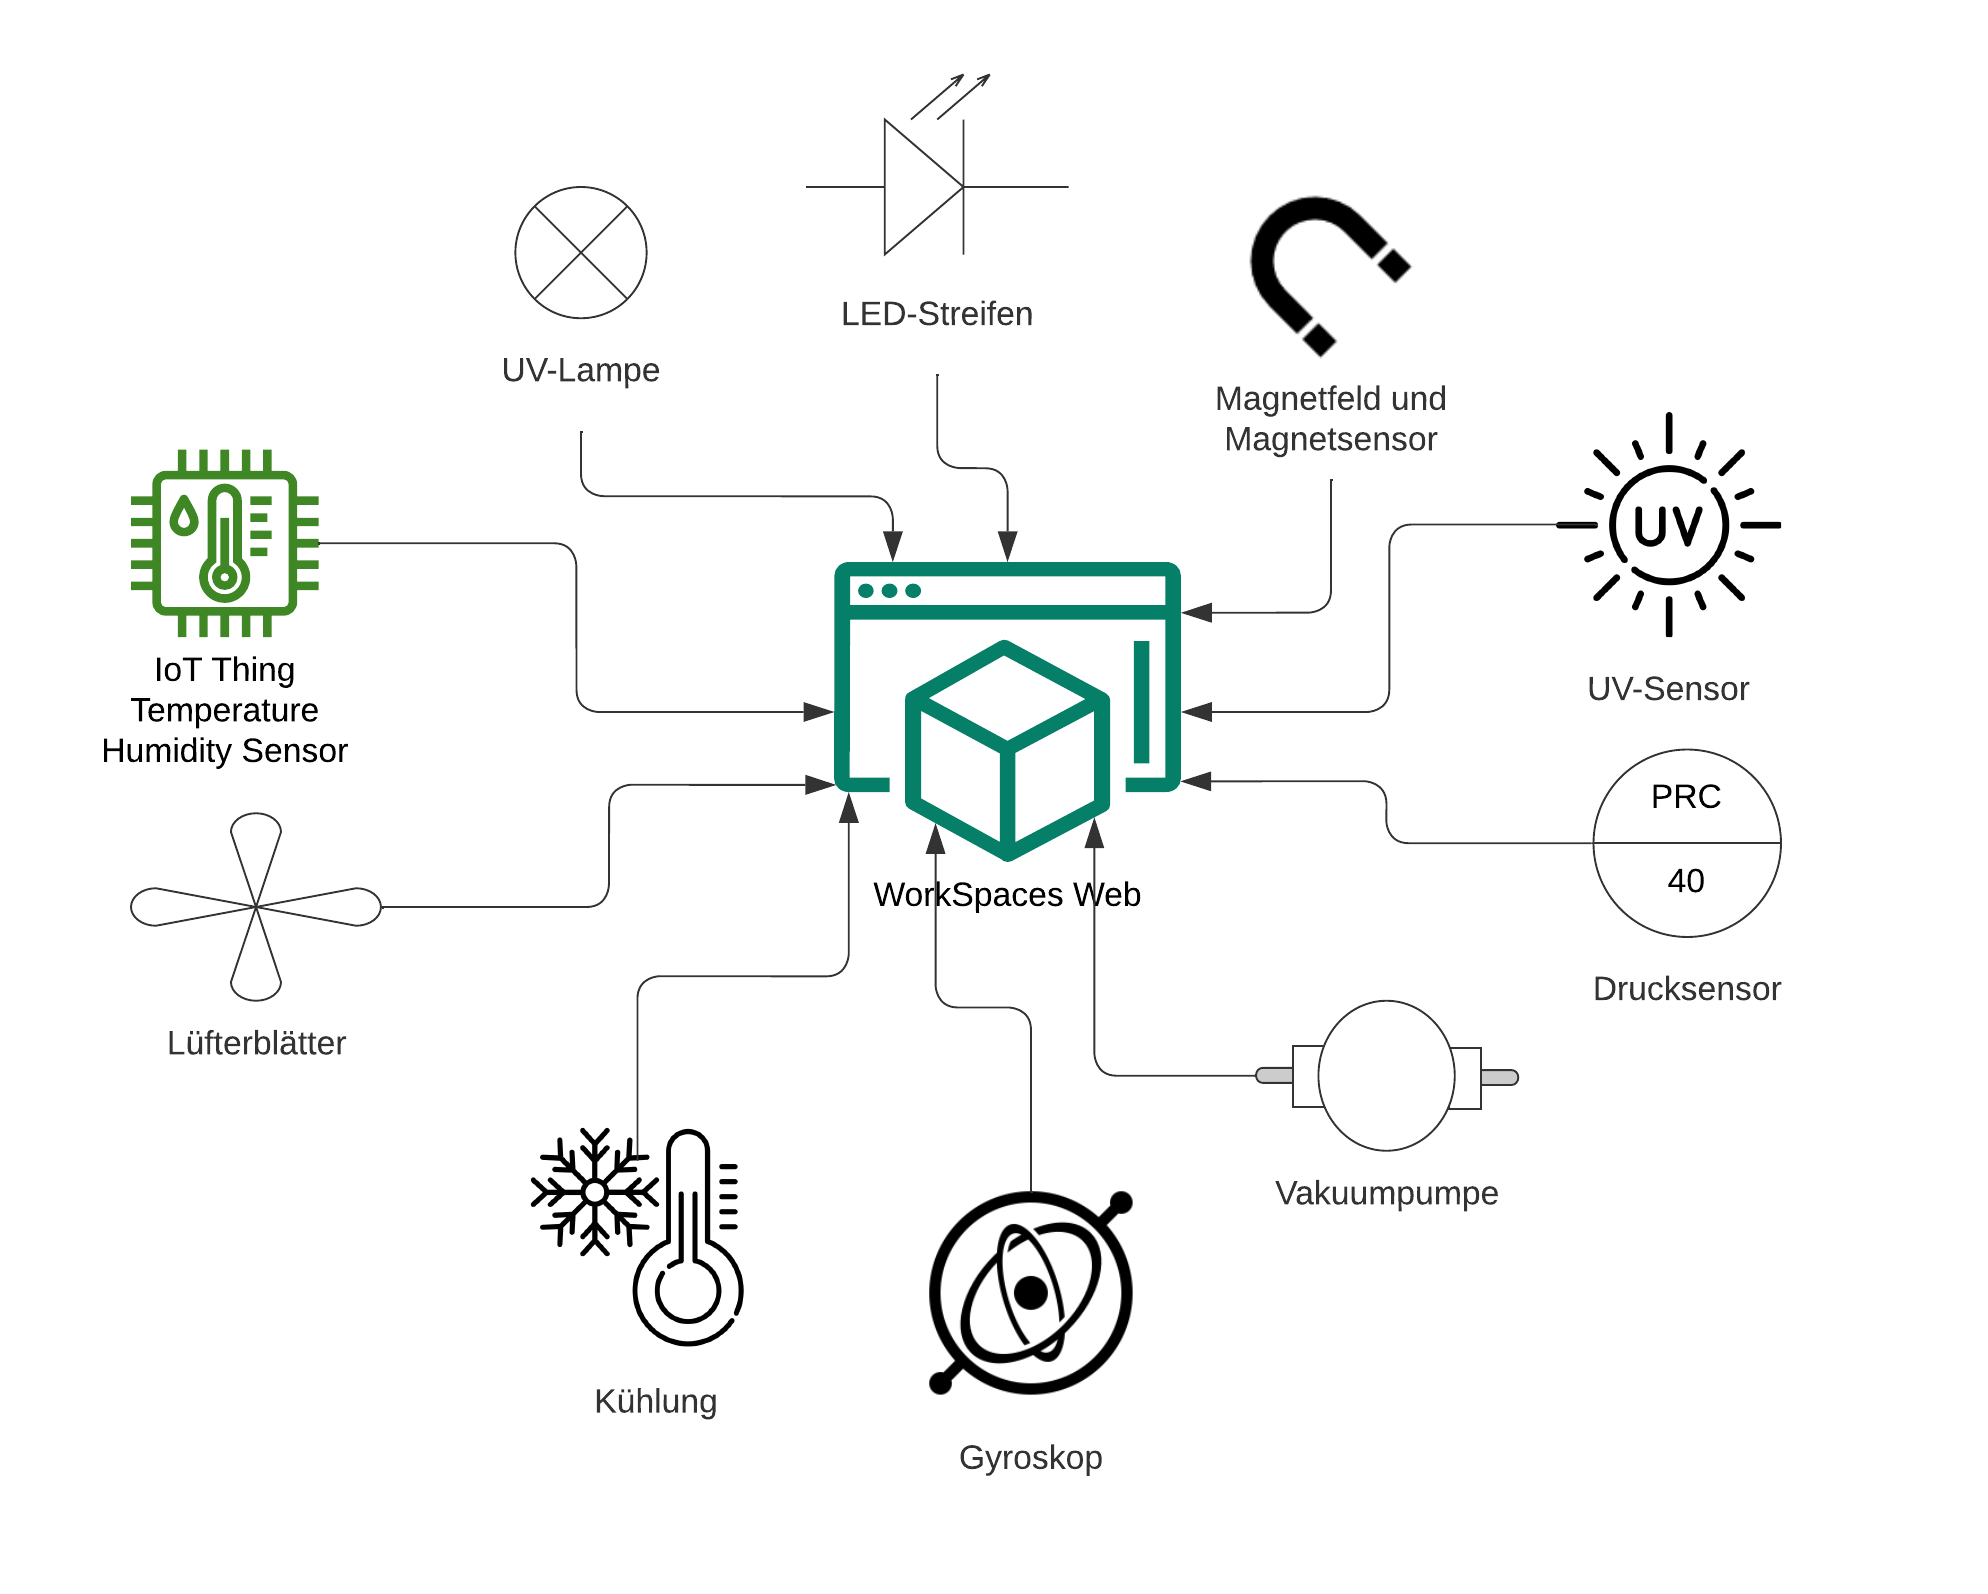
\includegraphics[scale=0.2]{image/blockgesamt.png}
	\caption{Blockschaltbild}
	\label{fig:enter-label}
\end{figure}

Das Setup, mit dem die Teststation gesteuert wird, soll einfach zu bedienen sein. Die Datenauslesung und die Ansteuerung der Geräte sollen in der selben Web-Applikation erfolgen. 
\newpage
\subsubsection{Ziele \textit{Must-Have}}
\begin{itemize}
    \item Rotation des Satellit
    \item Messen der folgenden Auswirkungen auf den CubeSat
    \begin{itemize}
        \item Magnetfeld
        \item Temperatur
        \item UV-Strahlung 
    \end{itemize}
    \item Datenauslesung 
    \item Benutzerfreundliche Bedienoberfläche
\end{itemize}

\subsubsection{Optionale Ziele \textit{Nice-to-Have}}
\begin{itemize}
    \item  Eine Vorrichtung, um ein Vakuum zu erzeugen.
    \item  Auswirkungen von Vibrationen auf den CubeSat
\end{itemize}

\subsection{ Meilensteine}

\begin{table}[h]
    \centering
\begin{tabular}{  l | c | c  } 
  
  \textbf{ Meilenstein} & \textbf{ zu erledigende Arbeit} & \textbf{ bis}\\
  \vspace{2mm}
   \\
   Gehäuse & \parbox{5cm}{Konstuktion und Aufbau des Gehäuses für die Teststation}   & 06.11.2023 \\ 
  \vspace{2mm}
   \\
   Testkammer & \parbox{5cm}{Sensoren einbauen \\ Gyroskop aufbauen \\  Vorrichtung für Vakuum \\ Kühlung \\ UV-Lampe }& 10.02.2024 \\ 
  \vspace{2mm}
   \\
   Daten ein- und auslesen & \parbox{5cm}{Programm für Ein- und Auslesen der Sensoren\\ verschiedene Sendemethoden testen} & 12.02.2024 \\ 
  \vspace{2mm}
   \\
   Limits Testen & Kritische Werte testen & 01.03.2024\\
  \vspace{2mm}
   \\
   Abgabe Diplomarbeit & Dokumentation abgeben & 20.03.2024\\
 
\end{tabular}
    \caption{Meilensteine}
\end{table}
\newpage
\subsection{ Team}
\subsubsection{Teammitglieder}

\begin{figure}[h]
  \centering
  \begin{adjustbox}{valign=c}
    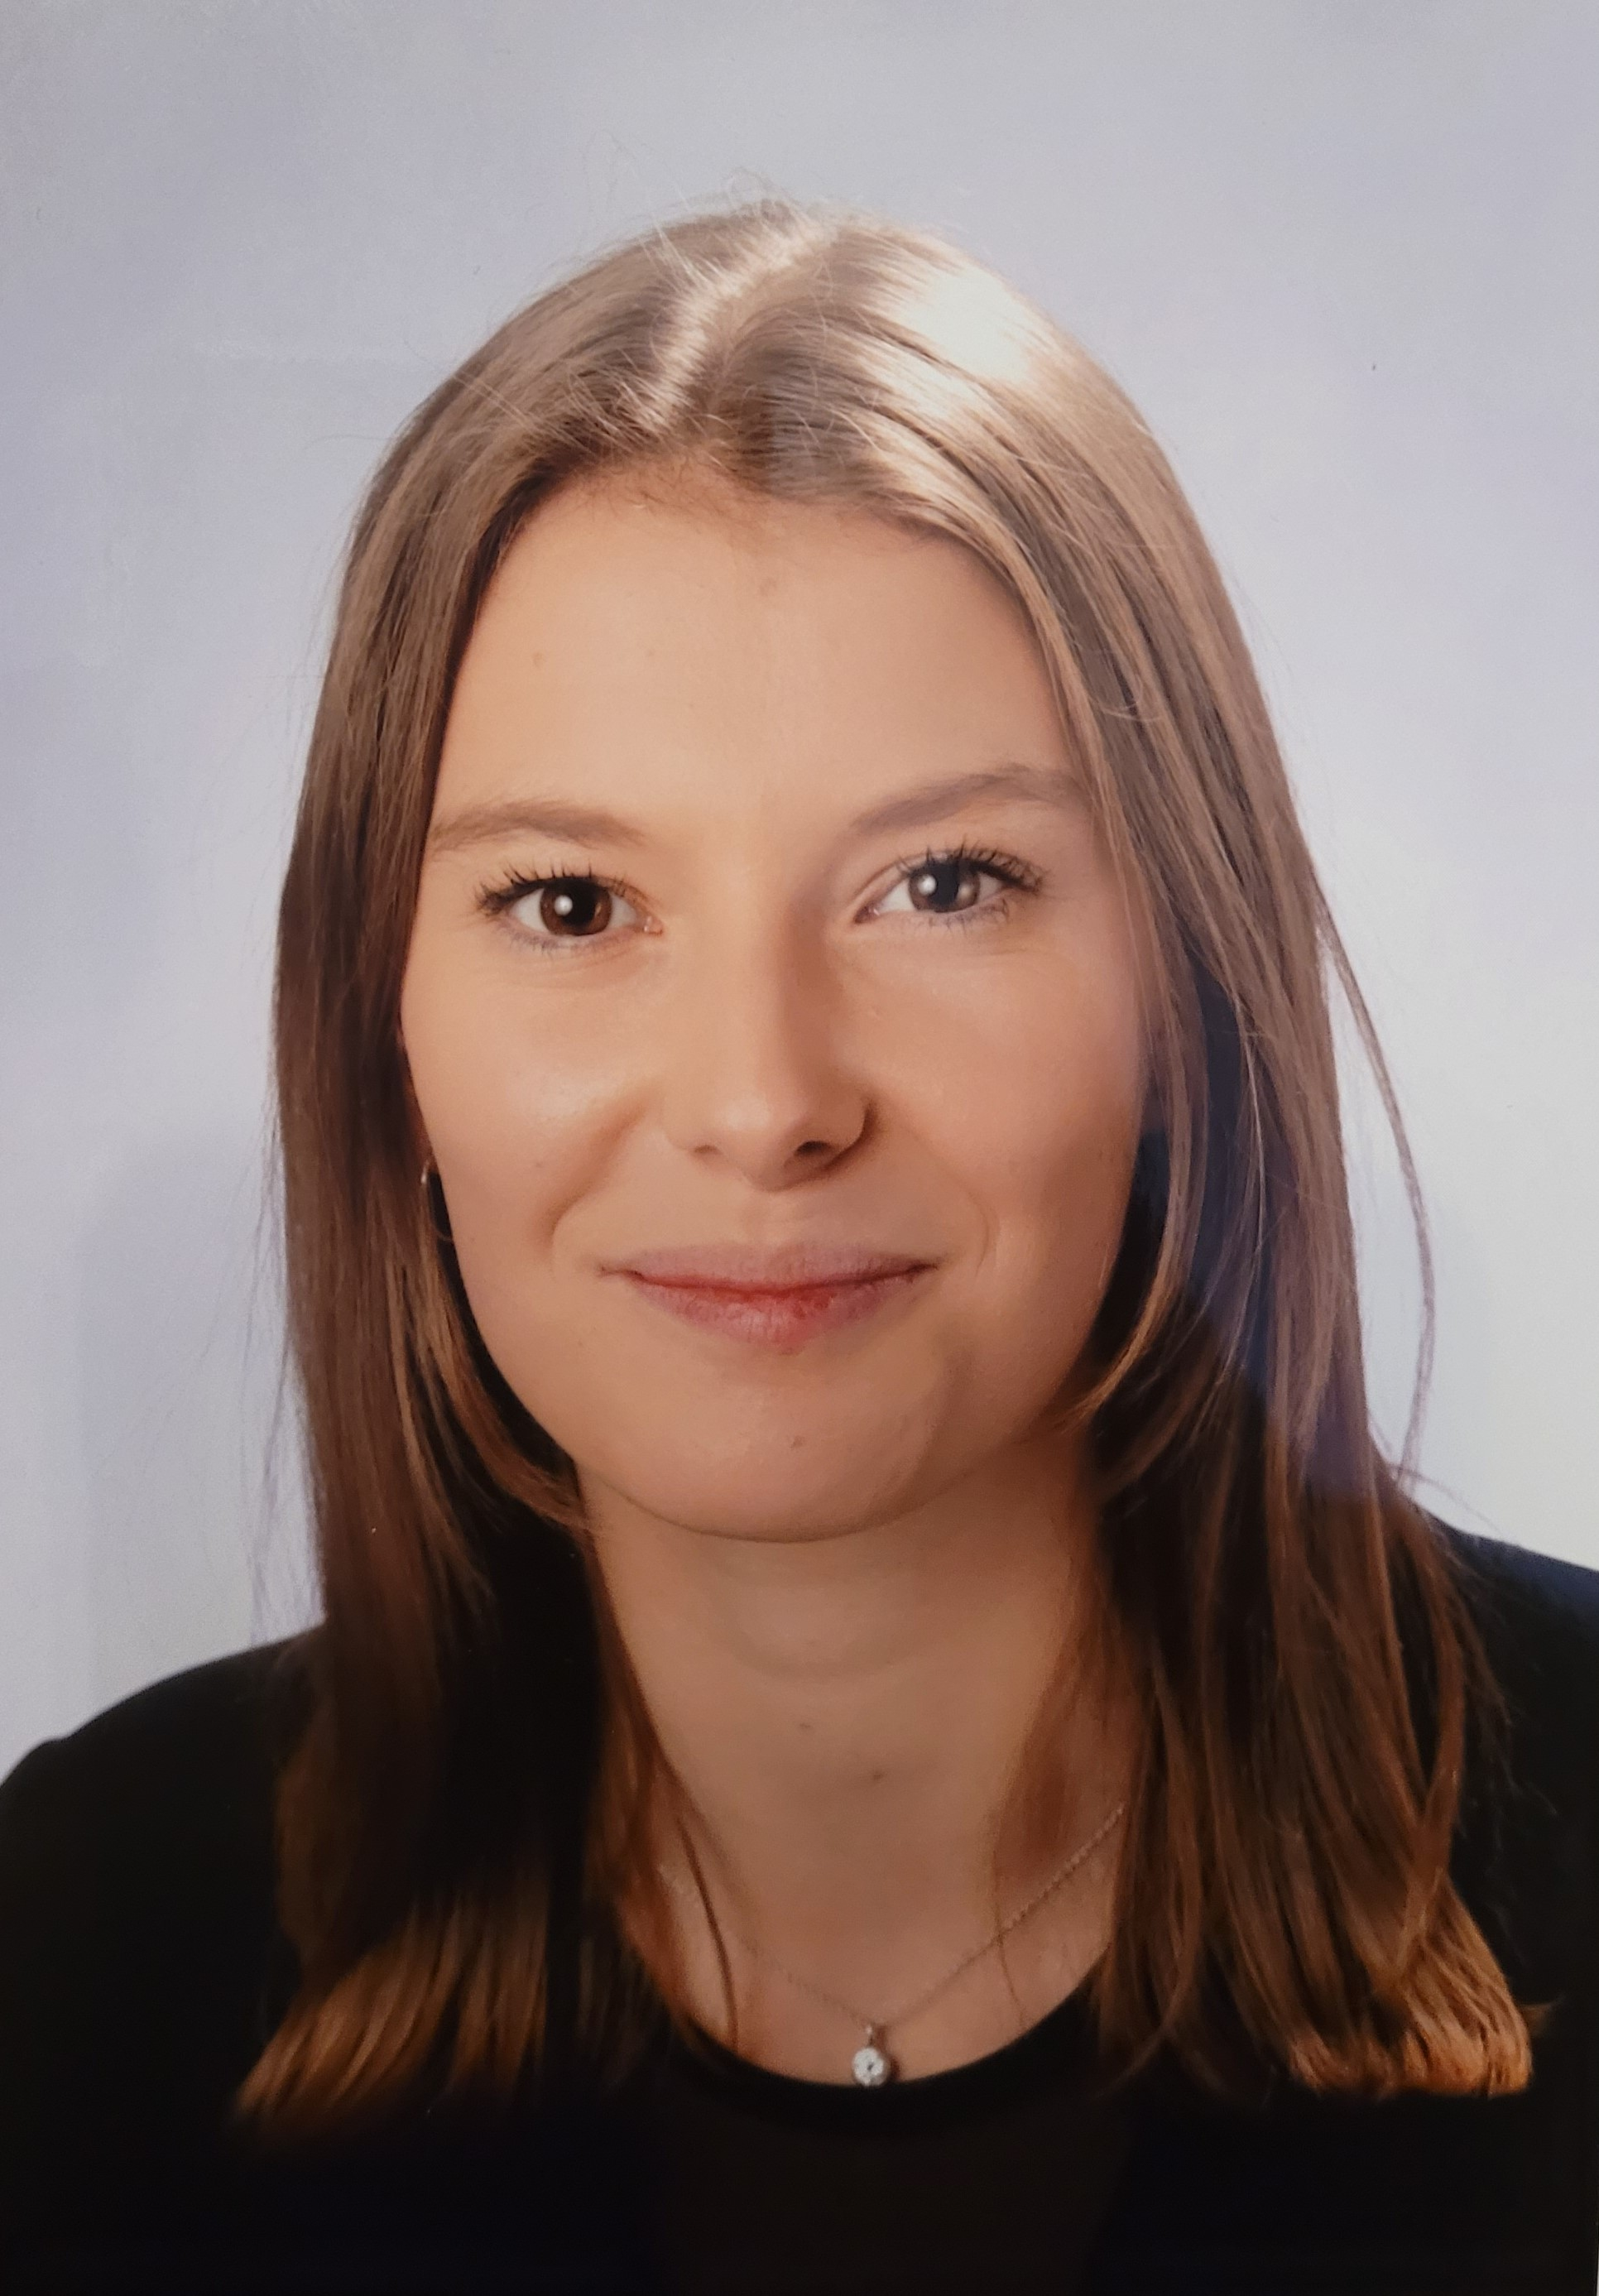
\includegraphics[scale=0.06]{image/Sophia.jpg}
  \end{adjustbox}
  \hfill
  \begin{minipage}[b]{0.7\textwidth}
    \textbf{\nameSH} \\ 5BHEL
  \end{minipage}
  \captionsetup{justification=raggedright,singlelinecheck=false}
  \caption{\nameSH}
\end{figure}

\begin{figure}[h]
  \centering
  \begin{adjustbox}{valign=c}
    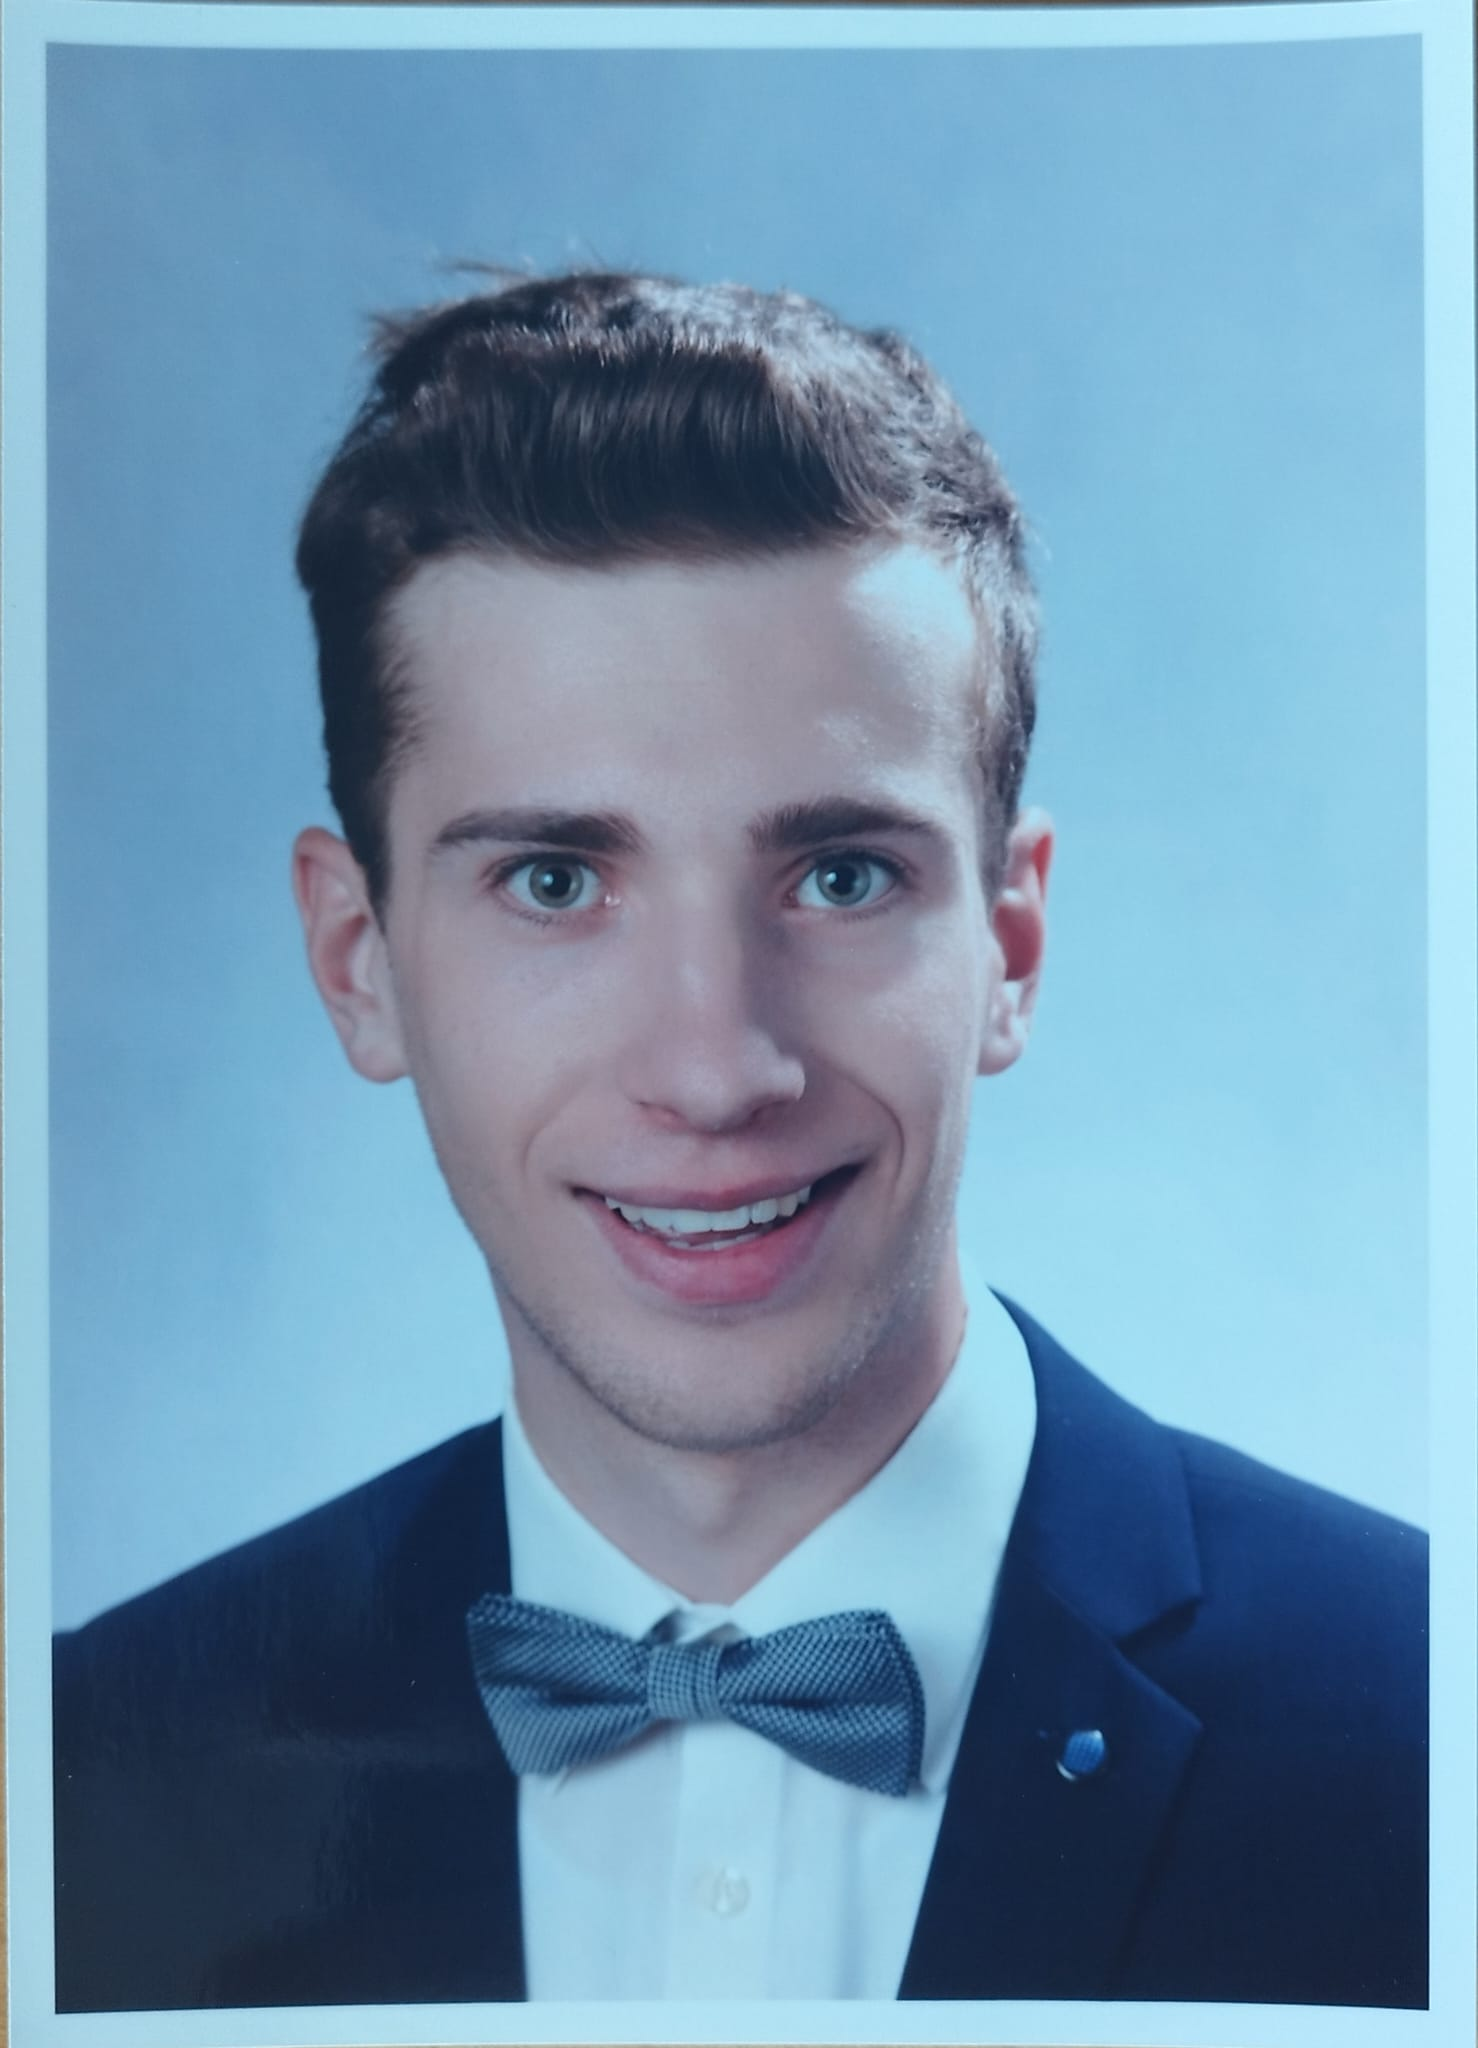
\includegraphics[scale=0.08]{image/Julius.jpeg}
  \end{adjustbox}
  \hfill
  \begin{minipage}[b]{0.7\textwidth}
    \textbf{\nameJS} \\ 5BHEL
  \end{minipage}
  \captionsetup{justification=raggedright,singlelinecheck=false}
  \caption{\nameJS}
\end{figure}
\newpage
\begin{figure}[h]
  \centering
  \begin{adjustbox}{valign=c}
    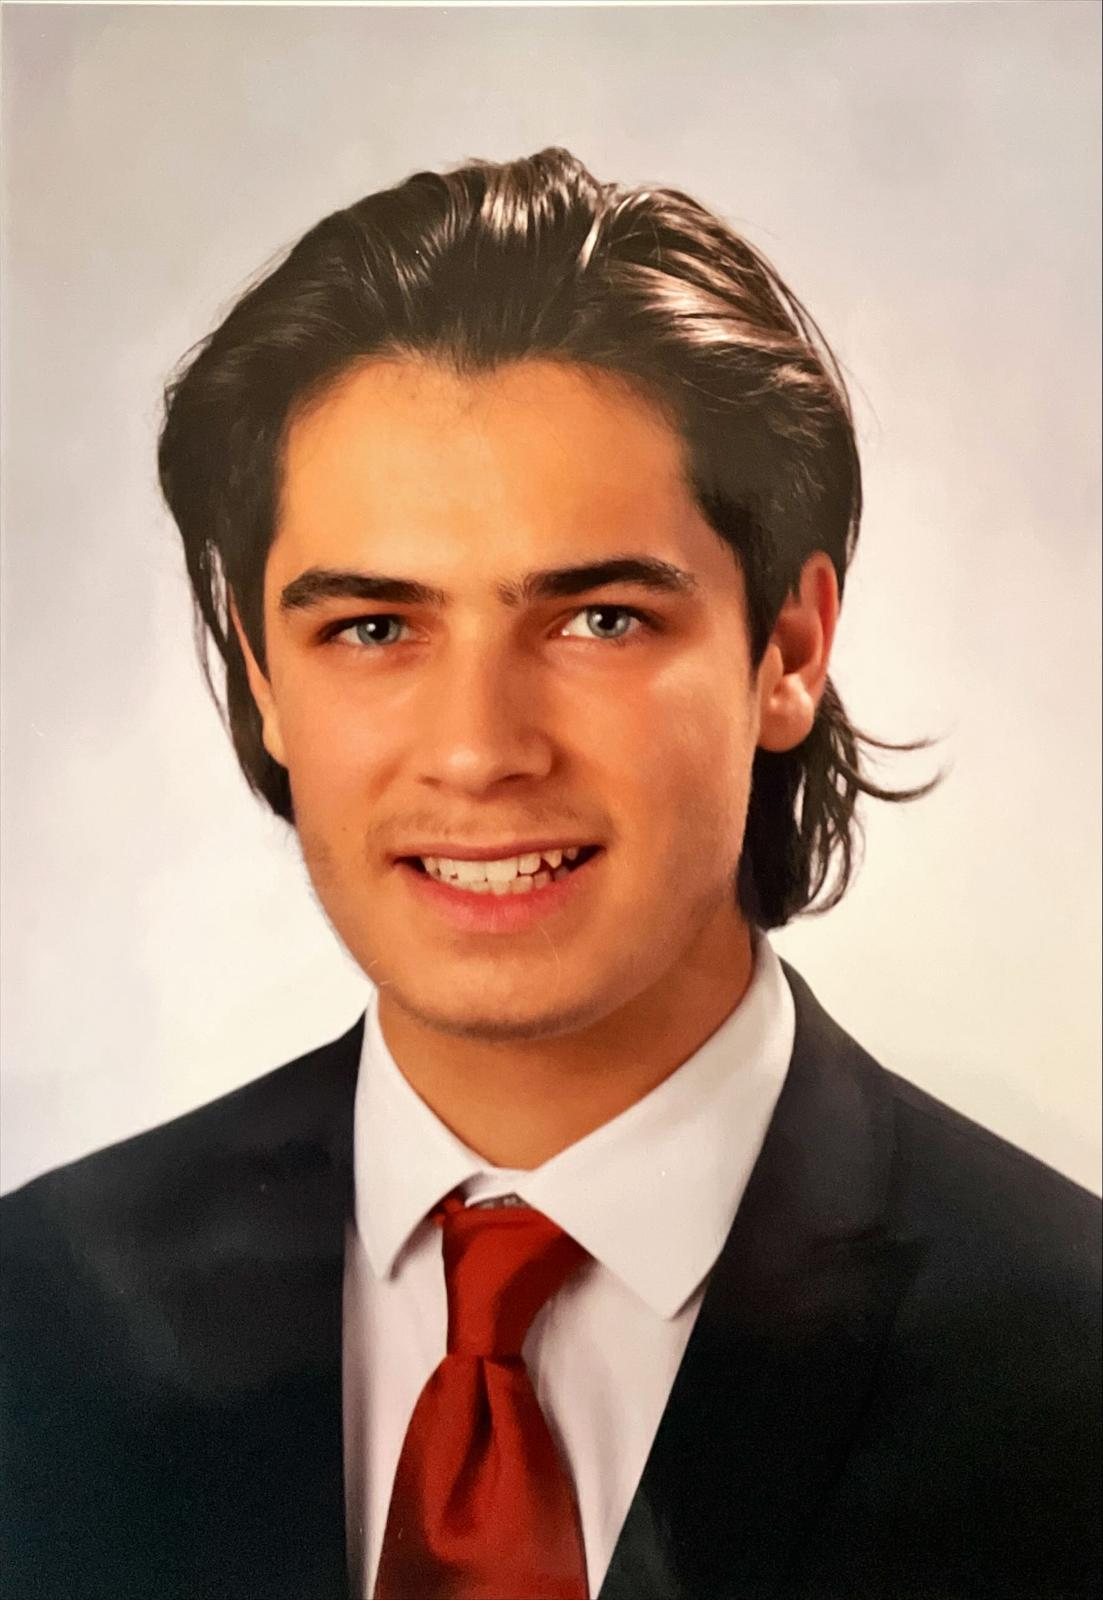
\includegraphics[scale=0.105]{image/consti.jpg}
  \end{adjustbox}
  \hfill
  \begin{minipage}[b]{0.7\textwidth}
    \textbf{\nameCZ} \\ 5BHEL
  \end{minipage}
  \captionsetup{justification=raggedright,singlelinecheck=false}
  \caption{\nameCZ}
\end{figure}

\begin{figure}[h]
  \centering
  \begin{adjustbox}{valign=c}
    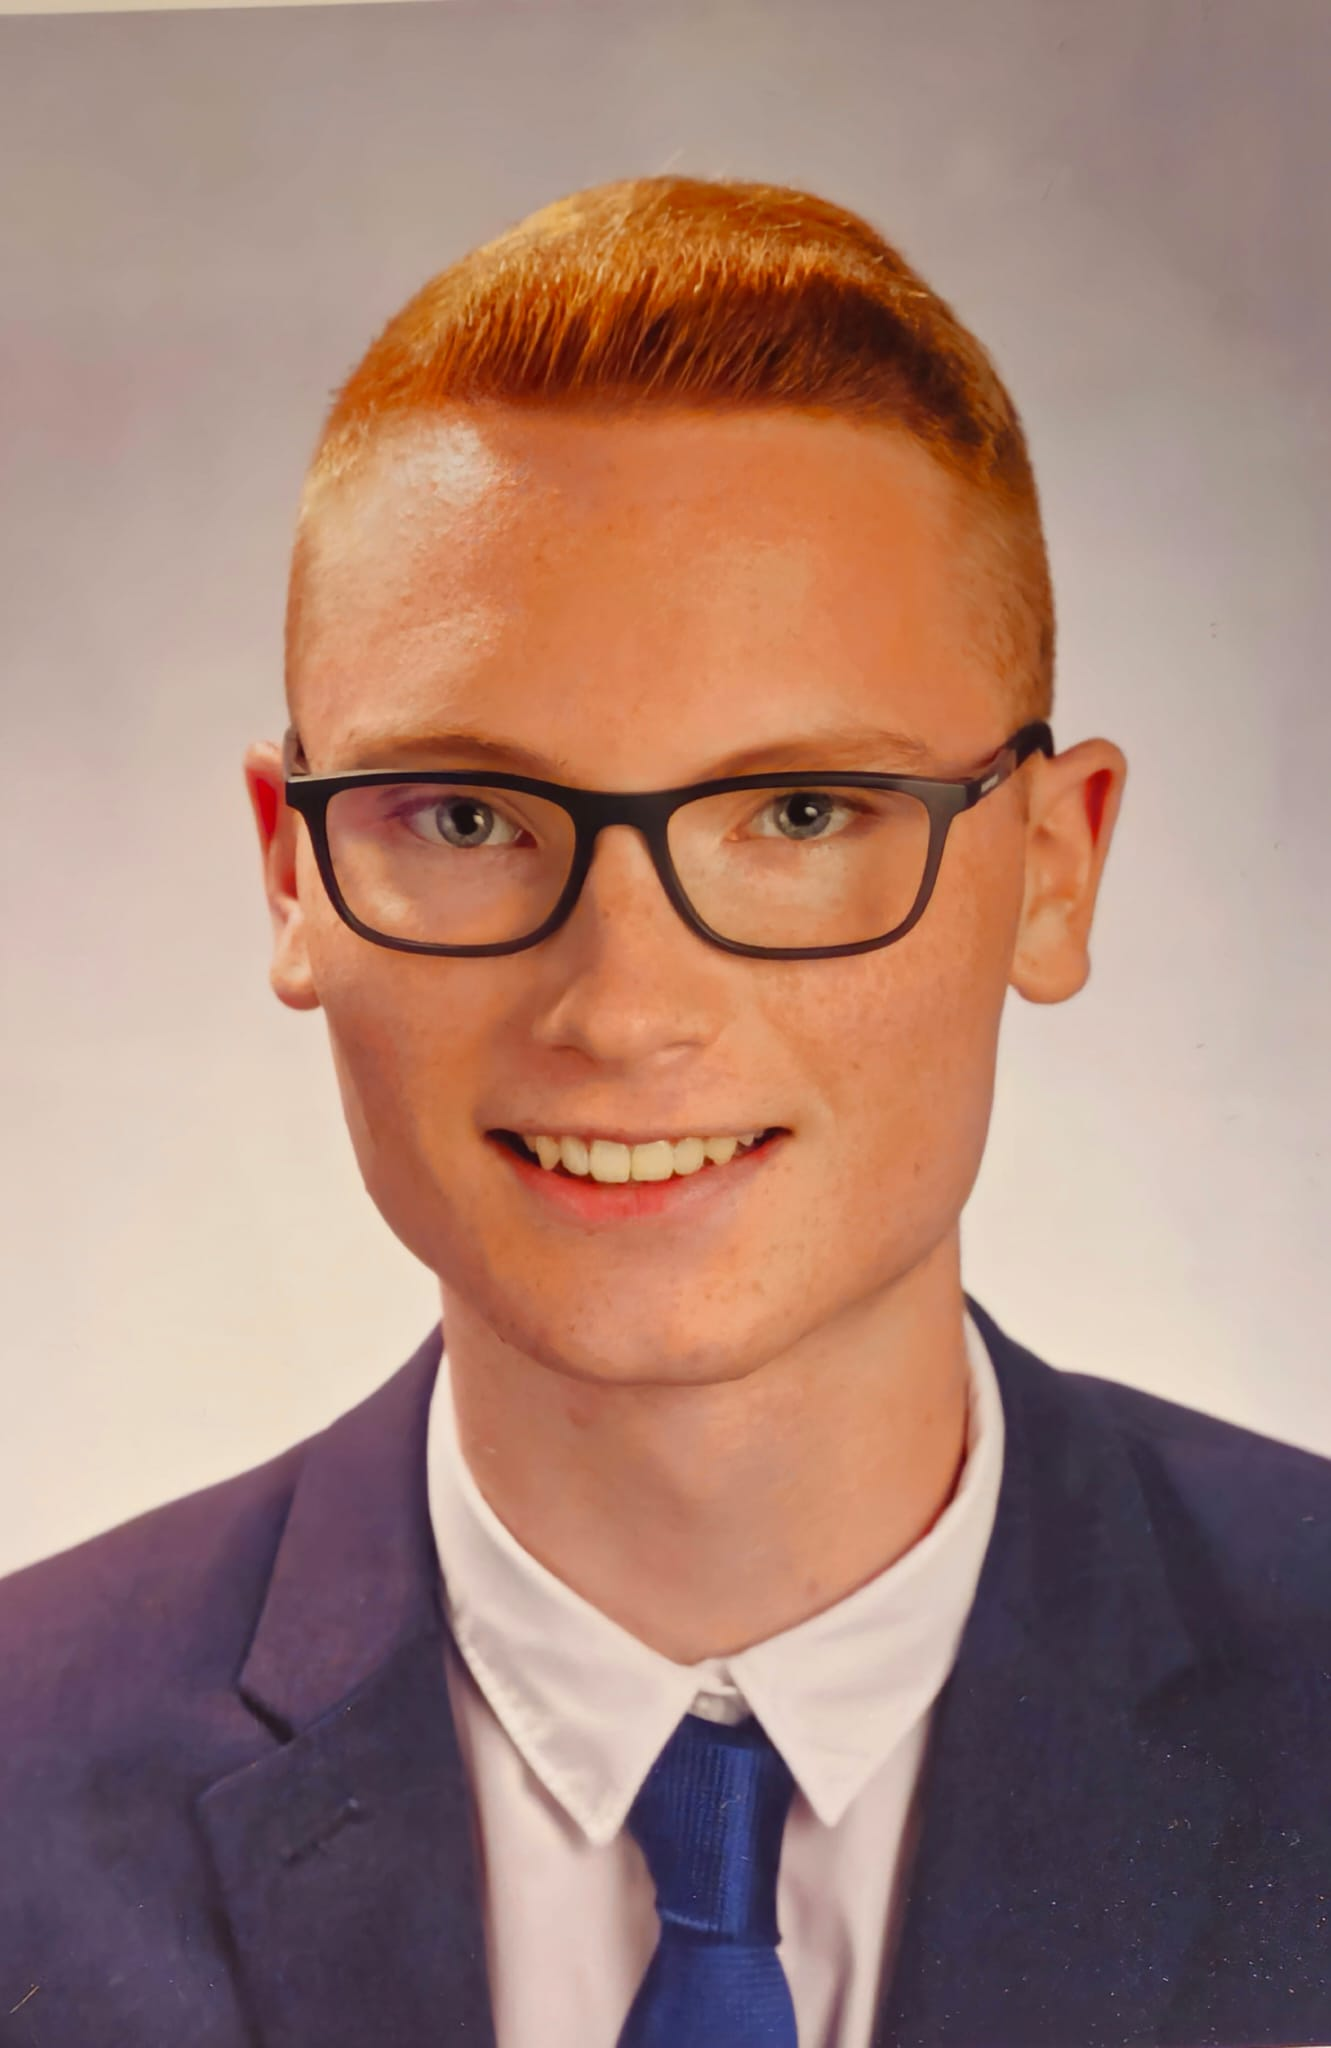
\includegraphics[scale=0.09]{image/Bellai.jpeg}
  \end{adjustbox}
  \hfill
  \begin{minipage}[b]{0.7\textwidth}
    \textbf{\nameSB} \\ 5AHEL
  \end{minipage}
  \captionsetup{justification=raggedright,singlelinecheck=false}
  \caption{\nameSB}
\end{figure}
\newpage
\subsubsection{ Betreungslehrer}
\begin{figure}[h]
  \centering
  \begin{adjustbox}{valign=c}
    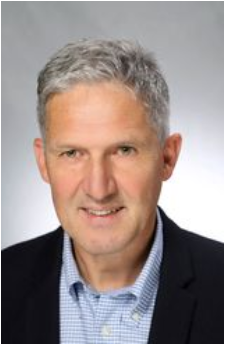
\includegraphics[scale=1]{image/Bischof.png}
  \end{adjustbox}
  \hfill
  \begin{minipage}[b]{0.7\textwidth}
    \textbf{Dipl. Ing. Gerold Bischof} \\ gerold.bischof(at)htl-rankweil.at
  \end{minipage}
  \captionsetup{justification=raggedright,singlelinecheck=false}
  \caption{Diplo. Ing. Gerold Bischof}
\end{figure}

\newpage

